

\documentclass{article}
\usepackage[utf8]{inputenc}
\usepackage{csquotes}
\usepackage[romanian]{babel}
\usepackage[hidelinks]{hyperref}

\usepackage{listings}
\usepackage{tabto}
\usepackage{graphicx}
\usepackage{xcolor}
\usepackage{float}
\lstset{basicstyle=\ttfamily\footnotesize, breaklines=true}
\lstdefinestyle{sharpc}{language=[Sharp]C, frame=lr, rulecolor=\color{blue!80!black}}


\begin{document}
	
	\title{Generarea Procedurală a
		Dungeon-urilor în Unity}
	\author{Cordunianu Radu \and Legian Andrei \and Tamaș Iulia \and Mujdar Milan \and Modreanu Maria \and Ibadula Adel}
	\date{}
	\maketitle
	
	\section{Introducere}
	\tab  Generarea procedurală reprezintă crearea algoritmică a conținutului (niveluri, hărți, obiecte) în mod aleator sau pseudo-aleator, evitând proiectarea manuală a fiecărui element.\cite{wiki-procgen} În contextul jocurilor video, un dungeon se referă la un labirint cu camere și coridoare populate de inamici, comori și capcane. Un dungeon generat procedural este de obicei un mediu labirintic interconectat, cu provocări și recompense
	plasate aleator, permițând explorare liberă dar menținând un progres controlat de dificultate. \cite{intro}
	
	Scopul acestui proiect este să implementeze mai mulți algoritmi de generare a dungeon-urilor 2D în Unity. Proiectul demonstrează trei abordări
	principale:
	\begin{itemize}
		\item \textbf{Simple Random Walk} – un algoritm simplu de „plimbare aleatorie” a unui agent prin spațiu, care generează un layout de tip peșteră (cu coridoare întortocheate și spații deschise)
		\item \textbf{Random Walk Corridor (Corridor-First)} – întâi se generează coridoare liniare prin random walk, apoi se adaugă camere la capetele sau de-a lungul acestor coridoare
		\item \textbf{Binary Space Partitioning (Room-First)} – se subîmparte recursiv spațiul în secțiuni (camere) și apoi camerele sunt conectate cu coridoare, asigurând un layout structurat, fără suprapuneri
	\end{itemize}
	
	 Toate cele trei generatoare sunt implementate ca clase MonoBehaviour în Unity, derivând dintr-o clasă abstractă comună.  Fiecare generator
	 procedural suprascrie metoda abstractă de rulare a algoritmului, oferind propria strategie de construire a dungeon-ului. Rezultatul este redat grafic pe un Tilemap Unity, folosind un tileset pixel-art pentru podele,
	 pereți și obiecte de decor.
	 \begin{figure}
	 	\centering
	 	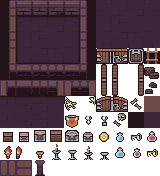
\includegraphics{Dungeon_Tileset.png}
	 	\caption{Tileset-ul folosit în cadrul proiectului}
	 \end{figure}
	 \newpage
	 
	\section{Simple Random Walk} 
	\tab Algoritmul \textbf{Simple Random Walk} (cunoscut și ca `drunkard's walk'') folosește o celulă de start care se deplasează aleator (sus, jos, stânga, dreapta), marcând podeaua dungeon-ului pe măsură ce avansează. Rezultatul este o rețea de celule conectate, cu aspect neregulat, similar cu o peșteră. Se poate rula de mai multe ori din puncte diferite pentru a crea zone extinse. \cite{rogue-randomwalk}
	
	 \newline
	 
	\textbf{Implementare în Unity:}
	\begin{itemize}
		\item Clasa \emph{SimpleRandomWalkDungeonGenerator} implementează algoritmul.
		\item Parametrii precum numărul de iterații și lungimea plimbării sunt setați într-un \textit{ScriptableObject}.
		\item ”Celula” pornește dintr-o poziție și creează o mulțime de coordonate \textit{(HashSet<Vector2Int>)} pentru podea.
		\item Punctul de start pentru fiecare iterație este ales aleator din zonele deja explorate.
		
		
	\end{itemize}
\newpage
\lstset{style=sharpc}	
\begin{lstlisting}[caption={Implementarea algoritmului Simple Random Walk din cadrul proiectului.}, 
	basicstyle=\ttfamily\small, 
	tabsize=4, 
	columns=fullflexible,
	frame=single,
	breaklines=true
	]
protected HashSet<Vector2Int> RunRandomWalk(SimpleRandomWalkSO parameters, Vector2Int startPosition)
{
	var currentPosition = startPosition;
	HashSet<Vector2Int> floorPositions = new HashSet<Vector2Int>();
	
	for (int i = 0; i < parameters.iterations; i++)
	{

		var path = ProceduralGenerationAlgorithms.SimpleRandomWalk(currentPosition, parameters.walkLength);
		
		
		floorPositions.UnionWith(path);

		if (parameters.startRandomlyEachIteration)
		currentPosition = floorPositions.ElementAt(Random.Range(0, floorPositions.Count));
	}
	
	return floorPositions;
}

\end{lstlisting}

 \newline
 
	\textbf{Integrare în Unity}
	
	\textit{După generare:}
	\begin{itemize}
		\item Se curăță tilemap-ul:
							\begin{lstlisting}[
			basicstyle=\ttfamily\small, 
			tabsize=2, 
			columns=fullflexible,
			frame=single,
			breaklines=true
			]
		 tilemapVisualizer.Clear();
		\end{lstlisting}

		\item Se picteaza podeaua:
					\begin{lstlisting}[
			basicstyle=\ttfamily\small, 
			tabsize=2, 
			columns=fullflexible,
			frame=single,
			breaklines=true
			]
		 tilemapVisualizer.PaintFloorTiles(floorPositions);
		\end{lstlisting}

		\item 	Se generează pereții:	
			\begin{lstlisting}[
			basicstyle=\ttfamily\small, 
			tabsize=2, 
			columns=fullflexible,
			frame=single,
			breaklines=true
			]
		WallGenerator.CreateWalls(floorPositions, tilemapVisualizer);
		\end{lstlisting}

	\end{itemize}
	
	\textit{Rezultate și caracteristici:}
	\begin{itemize}
	\item  Structură neregulată și haotică, cu aspect natural.
	\item  Zonele pot include camere mari și coridoare înguste.
	\item  Flexibil și simplu de implementat.
	\item  Lipsa unei structuri logice de camere/coridoare – potrivit pentru medii de tip cavernă.
\end{itemize}



	\section{ Random Walk Corridor (Corridor-First)}
	\tab Algoritmul \textbf{Random Walk Corridor} este o variație simplificată, specializată pe generarea de coridoare drepte. În loc să schimbe direcția la fiecare pas, acest algoritm alege o direcție fixă la început și marchează în linie o serie de celule pe acea direcție. Cu alte cuvinte, se generează un coridor de lungime predefinită orientat aleatoriu (nord, sud, est sau vest). \cite{kaiser-corridor}
	Structura rezultată are un traseu clar, iar camerele oferă spații pentru obiecte și lupte.
	
	 \newline
	 
	\textbf{Implementare în Unity}
	
	Clasa folosită este {CorridorFirstDungeonGenerator}, care extinde SimpleRandomWalkDungeonGenerator. Are parametri specifici:
	\begin{itemize}
		\item corridorLength, corridorCount – controlează numărul și lungimea segmentelor.
		\item roomPercent – procent din capetele coridoarelor care vor genera camere.
		\item ItemPlacementHelper – plasează inamici și obiecte.
		
	\end{itemize}
	\lstset{style=sharpc}	
	\begin{lstlisting}[caption={Implementarea algoritmului Simple Random Walk din cadrul proiectului.}, 
		basicstyle=\ttfamily\small, 
		tabsize=4, 
		columns=fullflexible,
		frame=single,
		breaklines=true
		]
private List<List<Vector2Int>> CreateCorridors(HashSet<Vector2Int> floorPositions, HashSet<Vector2Int> potentialRoomPositions)
{
	var currentPosition = startPosition;
	potentialRoomPositions.Add(currentPosition);
	
	List<List<Vector2Int>> corridors = new List<List<Vector2Int>>();
	
	for (int i = 0; i < corridorCount; i++)
	{
		var corridor = ProceduralGenerationAlgorithms.RandomWalkCorridor(currentPosition, corridorLength);
		corridors.Add(corridor);
		currentPosition = corridor[corridor.Count - 1];
		potentialRoomPositions.Add(currentPosition);
		floorPositions.UnionWith(corridor);
	}
	
	corridorPositions = new HashSet<Vector2Int>(floorPositions);
	return corridors;
}

		
	\end{lstlisting}
	
	Se creează o serie de coridoare drepte (aleator orientate), iar capetele lor sunt reținute pentru a deveni camere posibile.

	\newpage
	\textbf{Adăugarea camerelor}
	
	Un subset aleator din capetele de coridor devine punct de start pentru camere generate prin plimbare aleatorie (RunRandomWalk). Aceasta oferă formă neregulată camerelor:
	\lstset{style=sharpc}	
	\begin{lstlisting}[
		basicstyle=\ttfamily\small, 
		tabsize=2, 
		columns=fullflexible,
		frame=single,
		breaklines=true
		]
		var room = RunRandomWalk(randomWalkParameters, roomCenter);
	\end{lstlisting}
	
	\textbf{Plasarea elementelor interactive}
	
	Obiectele și inamici sunt plasați doar în camere, nu pe coridoare, folosind:
	\lstset{style=sharpc}	
	\begin{lstlisting}[
		basicstyle=\ttfamily\small, 
		tabsize=2, 
		columns=fullflexible,
		frame=single,
		breaklines=true
		]
itemPlacementHelper.Initialize(allRoomPositions, roomPositionsWithoutCorridors);

itemPlacementHelper.PlaceItems();
itemPlacementHelper.PlaceEnemies();
	\end{lstlisting}
	
	
	\section{Partiționarea binară a spațiului (Binary Space Partitioning)}
	\tab Această metodă folosește un algoritm de partiționare binară a spațiului (BSP) pentru a împărți harta în dreptunghiuri disjuncte (camere), apoi le conectează prin coridoare. Este o abordare „top-down”, care oferă maxim control asupra formei și distribuției camerelor, ideală pentru dungeon-uri structurate, de tip temniță clasică. \cite{rogue-bsp} \cite{eskerda-bsp}
	
	  \newline
	
	\textbf{Implementare în Unity}
	
	Clasa \textit{RoomFirstDungeonGenerator} extinde \textit{SimpleRandomWalkDungeonGenerator}. Parametri cheie:
	\begin{itemize}
		\item dungeonWidth, dungeonHeight – dimensiunile totale ale hărții.
		\item minRoomWidth, minRoomHeight – limite pentru camere.
		\item offset – spațiu liber între marginea zonei și cameră.
		\item randomWalkRooms – controlează dacă se generează camere dreptunghiulare sau organice.
	\end{itemize}
	\newpage
	\textbf{1. Partiționarea spațiului}
	Spațiul este împărțit recursiv în 2 zone, până când fiecare zonă este suficient de mică pentru a deveni o cameră:
		\lstset{style=sharpc}	
	\begin{lstlisting}[
		basicstyle=\ttfamily\small, 
		tabsize=2, 
		columns=fullflexible,
		frame=single,
		breaklines=true
		]
var roomsList = ProceduralGenerationAlgorithms.BinarySpacePartitioning(
	new BoundsInt(
		Vector3Int.zero,
		new Vector3Int(dungeonWidth, dungeonHeight, 0)
	),
	minRoomWidth,
	minRoomHeight
);


	\end{lstlisting}
	\tab Rezultatul este o listă de BoundsInt, fiecare reprezentând o zonă de cameră potențială.
	
	 \newline
		\textbf{2. Crearea camerelor}
	
	Se creează două tipuri de camere:
	\begin{itemize}
		\item 	Camere dreptunghiulare simple.
		\lstset{style=sharpc}	
		\begin{lstlisting}[
			basicstyle=\ttfamily\small, 
			tabsize=2, 
			columns=fullflexible,
			frame=single,
			breaklines=true
			]
			for (int col = offset; col < room.size.x - offset; col++)
			for (int row = offset; row < room.size.y - offset; row++)
			floor.Add(room.min + new Vector2Int(col, row));
			
			
			
		\end{lstlisting}
		\item Se folosește un random walk pentru a genera camere neregulate
				\lstset{style=sharpc}	
		\begin{lstlisting}[
			basicstyle=\ttfamily\small, 
			tabsize=2, 
			columns=fullflexible,
			frame=single,
			breaklines=true
			]
var roomCenter = Vector2Int.RoundToInt(roomBounds.center);
var roomFloor = RunRandomWalk(randomWalkParameters, roomCenter);
		
		\end{lstlisting}
	\end{itemize}
	\tab Doar tile-urile care rămân în interiorul zonei sunt păstrate (se aplică filtrare după offset).
	
	 \newline
	 \textbf{3. Conectarea camerelor} \newline
	 
	 \tab Se aleg centrele camerelor \textit{Vector2Int.RoundToInt(room.center)}, apoi sunt conectate între ele cu coridoare în formă de „L”:
	 
	 
				\lstset{style=sharpc}	
\begin{lstlisting}[
	basicstyle=\ttfamily\small, 
	tabsize=2, 
	columns=fullflexible,
	frame=single,
	breaklines=true
	]
CreateCorridor(pointA, pointB);
\end{lstlisting}
\newpage
Aceasta construiește un traseu ortogonal: se merge vertical până la același Y, apoi orizontal până la X-ul țintă.
				\lstset{style=sharpc}	
\begin{lstlisting}[
	basicstyle=\ttfamily\small, 
	tabsize=2, 
	columns=fullflexible,
	frame=single,
	breaklines=true
	]
while (position.y != destination.y)
{
	position += (destination.y > position.y) ? Vector2Int.up : Vector2Int.down;
	corridor.Add(position);
}
while (position.x != destination.x)
{
	position += (destination.x > position.x) ? Vector2Int.right : Vector2Int.left;
	corridor.Add(position);
}

\end{lstlisting}
\tab Rezultatul este un graf conex, fără cicluri, toate camerele fiind accesibile.

  \newline
\textbf{Caracteristici ale rezultatului}
\begin{itemize}
	\item Layout ordonat, cu camere distincte și coridoare directe.
	\item Permite control asupra dimensiunii și formei fiecărei camere.
	\item Cu \textit{randomWalkRooms}, se obțin forme mai organice.
	\item Fără bucle – doar un singur drum între oricare două camere.
\end{itemize}
\newpage
	\section{Gameplay și impactul generării procedurale}
	
		\tab Gameplay-ul propus în acest proiect se bazează pe explorare, luptă și progresie prin spații necunoscute.
		Jucătorul controlează un personaj echipat cu o baghetă magică cu care poate ataca inamicii. Proiectilele lansate trebuie să atingă ținta de mai multe ori pentru a o elimina. Pe hartă sunt răspândiți inamici de tip slime, care urmăresc jucătorul odată ce intră în raza lor vizuală, forțându-l să navigheze rapid și strategic prin camere și coridoare.


		\begin{figure}[H]
			\centering
			\includegraphics[width=\textwidth,height=\textheight,keepaspectratio]{image.png}
			\caption{Jucătorul împuscând multipli inamici}
		\end{figure}
		
		
		Pe lângă supraviețuire, jucătorul are un obiectiv clar: să găsească o cheie și ulterior să descopere ușa de ieșire, ambele amplasate aleator. Astfel, fiecare generație procedurală creează un mic puzzle de navigare și decizie.
		
		Pe hartă apar și două tipuri de cufere, cu recompense diferite:
		\begin{itemize}
			\item Cufărul simplu: \textit{5 monede}
			\item Cufărul mare: \textit{10 monede}
		\end{itemize}
		Totodată, într-unul dintre cuferele mari se află ascunsă cheia, de care jucătorul are nevoie.
		În plus, fiecare inamic învins aduce o monedă. 
				\begin{figure}[H]
			\centering
			\includegraphics[width=\textwidth,height=\textheight,keepaspectratio]{image2.png}
			\caption{Jucătorul aflandu-se în aceeași cameră cu cheia și ușa}
		\end{figure}
		
	\section{Concluzie}
\tab Proiectul de față demonstrează versatilitatea generării procedurale aplicate în Unity, folosind trei abordări algoritmice fundamentale: Simple Random Walk, Corridor-First și Binary Space Partitioning. Fiecare dintre acestea oferă avantaje specifice în funcție de tipul de nivel dorit, de la spații organice, la structuri semi-lineare sau dungeon-uri clar compartimentate.

Prin integrarea acestor algoritmi cu o logică de gameplay simplă, dar funcțională, proiectul reușește să creeze niveluri dinamice, navigabile și rejucabile, în care jucătorul este provocat să exploreze, să înfrunte inamici și să urmărească obiective strategice precum găsirea cheii și ieșirea din dungeon.
	\newpage
	\section{Bibliografie}
\begin{thebibliography}{6}
\bibitem{wiki-procgen} 
Procedural generation, Wikipedia (ultima accesare: 12 mai 2025). Disponibil online la: \url{https://en.wikipedia.org/wiki/Procedural_generation}

\bibitem{intro}Constructive Generation Methods for Dungeons and Levels
- Noor Shaker, Antonios Liapis, Julian Togelius, Ricardo Lopes și Rafael Bidarra. Disponibil la \url{https://antoniosliapis.com/articles/pcgbook_dungeons.php}


\bibitem{rogue-randomwalk} 
Random Walk Cave Generation, RogueBasin Wiki (articol, 2010). Algoritm \textit{drunkard's walk} pentru generarea de peșteri 2D. Disponibil la: \url{https://www.roguebasin.com/index.php/Random_Walk_Cave_Generation}

\bibitem{kaiser-corridor}
J. H. Kaiser, Corridor path generator algorithms, Preprint, (mai 2020). Disponibil la:  \url{https://www.researchgate.net/publication/341787742}

\bibitem{rogue-bsp} 
Basic BSP Dungeon generation, RogueBasin Wiki (articol). Prezentare a metodei de partiționare binară a spațiului pentru dungeon-uri, inclusiv conectarea camerelor prin coridoare. Disponibil la: \url{https://www.roguebasin.com/index.php/Basic_BSP_Dungeon_generation}

\bibitem{eskerda-bsp} 
Dungeon generation using BSP trees,eskerda.com (blog), 2013. Explicație a algoritmului BSP; descrie împărțirea recursivă și conectarea centrului regiilor surori. Disponibil la: \url{http://eskerda.com/bsp-dungeon-generation/}

\bibitem{gamasutra-tinykeep} 
A. Adonaac, Procedural Dungeon Generation Algorithm, GameDeveloper.com, 2015. Articol de blog ce detaliază algoritmul folosit în jocul *Tiny Keep* pentru generarea de dungeon-uri, oferind o perspectivă complementară asupra tehnicilor de mai sus. Disponibil la: \url{https://www.gamedeveloper.com/programming/procedural-dungeon-generation-algorithm}

\end{thebibliography}

\end{document}
